% CMS coordinate system (left) and pseudorapidity vs polar angle (right).
% Compile with: pdflatex cms_coordinates.tex  -> copy the PDF to figures/chapter_II/
\documentclass[tikz,border=4pt]{standalone}
\usepackage{amsmath}
\usetikzlibrary{arrows.meta,calc,angles,quotes}

\definecolor{cmsblue}{RGB}{31,90,166}
\definecolor{cmsred}{RGB}{200,40,40}
\definecolor{cmsgray}{RGB}{120,120,120}

\begin{document}
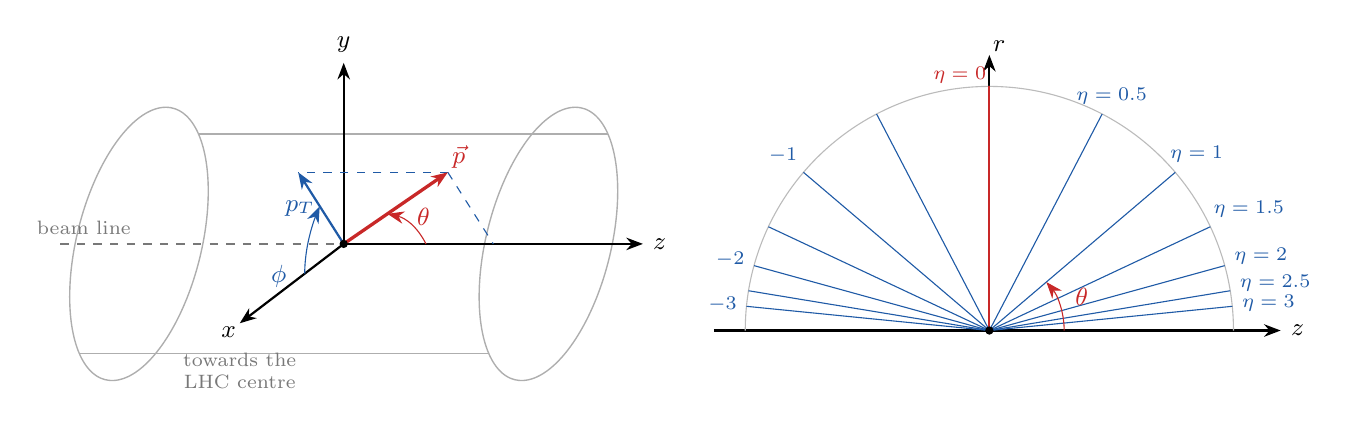
\begin{tikzpicture}[>={Stealth[length=6pt]}, font=\small]

% ------------------------------------------------------------------
% Left panel: 3D coordinate system (oblique projection)
%   z horizontal (beam), y vertical, x towards the viewer (lower left)
% ------------------------------------------------------------------
\begin{scope}[x={(-0.55cm,-0.42cm)}, y={(0cm,1cm)}, z={(1cm,0cm)}]
  \def\R{1.6}
  \def\L{2.6}
  % detector barrel (schematic cylinder)
  \draw[cmsgray!60, line width=0.5pt, domain=0:360, samples=90, smooth]
    plot ({\R*cos(\x)}, {\R*sin(\x)}, {-\L});
  \draw[cmsgray!60, line width=0.5pt, domain=0:360, samples=90, smooth]
    plot ({\R*cos(\x)}, {\R*sin(\x)}, {\L});
  \draw[cmsgray!60, line width=0.5pt] (-0.86*\R, 0.51*\R, -\L) -- (-0.86*\R, 0.51*\R, \L);
  \draw[cmsgray!60, line width=0.5pt] (0.86*\R, -0.51*\R, -\L) -- (0.86*\R, -0.51*\R, \L);

  % beam line
  \draw[cmsgray, line width=0.8pt, dashed] (0,0,-3.6) -- (0,0,-0.05);
  \node[cmsgray, anchor=south, font=\scriptsize] at (0,0,-3.3) {beam line};

  % axes
  \draw[->, thick] (0,0,0) -- (2.4,0,0) node[anchor=north east, inner sep=1pt] {$x$};
  \draw[->, thick] (0,0,0) -- (0,2.3,0) node[anchor=south] {$y$};
  \draw[->, thick] (0,0,0) -- (0,0,3.8) node[anchor=west] {$z$};
  \node[anchor=north, align=center, font=\scriptsize, cmsgray] at (2.4,-0.25,0) {towards the\\LHC centre};

  % momentum vector and its projections
  \coordinate (O) at (0,0,0);
  \coordinate (P) at (1.05,1.35,1.9);
  \coordinate (PT) at (1.05,1.35,0);
  \coordinate (PZ) at (0,0,1.9);
  \draw[cmsblue, dashed] (P) -- (PT);
  \draw[cmsblue, dashed] (P) -- (PZ);
  \draw[->, cmsblue, thick] (O) -- (PT) node[midway, anchor=east, inner sep=2pt] {$p_T$};
  \draw[->, cmsred, very thick] (O) -- (P) node[anchor=south west, inner sep=1pt] {$\vec{p}$};

  % azimuthal angle phi, in the x-y plane, from x
  \draw[cmsblue, domain=0:52, samples=30, smooth, ->]
    plot ({0.9*cos(\x)}, {0.9*sin(\x)}, 0);
  \node[cmsblue, anchor=north east, inner sep=1pt] at (1.25,0.3,0) {$\phi$};

  % polar angle theta, from z towards p
  \draw[cmsred, ->] ($(O)!0.55!(PZ)$) to[bend right=25] ($(O)!0.42!(P)$);
  \node[cmsred] at (0.25,0.45,1.15) {$\theta$};

  % interaction point
  \fill (O) circle (1.5pt);
\end{scope}

% ------------------------------------------------------------------
% Right panel: pseudorapidity vs polar angle in the (z, r) half-plane
% ------------------------------------------------------------------
\begin{scope}[xshift=8.2cm, yshift=-1.1cm]
  \def\Rr{3.1}
  \draw[->, thick] (-3.5,0) -- (3.7,0) node[anchor=west] {$z$};
  \draw[->, thick] (0,0) -- (0,3.5) node[anchor=south west, inner sep=1pt] {$r$};
  \draw[cmsgray!50] (\Rr,0) arc (0:180:\Rr);
  \foreach \e in {0.5,1,1.5,2,2.5,3} {
    \pgfmathsetmacro{\th}{2*atan(exp(-\e))}
    \draw[cmsblue] (0,0) -- (\th:\Rr);
    \draw[cmsblue] (0,0) -- (180-\th:\Rr);
    \node[cmsblue, font=\scriptsize, anchor={180+\th}] at (\th:\Rr) {$\eta=\e$};
  }
  \foreach \e in {1,2,3} {
    \pgfmathsetmacro{\th}{2*atan(exp(-\e))}
    \node[cmsblue, font=\scriptsize, anchor={-\th}] at (180-\th:\Rr) {$-\e$};
  }
  \draw[cmsred, thick] (0,0) -- (90:\Rr);
  \node[cmsred, font=\scriptsize, anchor=south east, inner sep=1pt] at (90:\Rr) {$\eta=0$};
  % example angle
  \pgfmathsetmacro{\thex}{2*atan(exp(-1.0))}
  \draw[cmsred, ->] (0.95,0) arc (0:\thex:0.95);
  \node[cmsred] at ({0.5*\thex}:1.25) {$\theta$};
  \fill (0,0) circle (1.5pt);
\end{scope}

\end{tikzpicture}
\end{document}
